\begin{multicols}{3}[\section{Light Fidelity}]

\rhead{Tizian Kurkamp}
\lfoot{08.05.2016}

\newrefsegment

\begin{tabular}{p{2,1 cm}p{2.7 cm}}
\textbf{Steckbrief}& \\
\end{tabular}
\rowcolors{1}{\topicolor!20}{}
\begin{tabular}{p{2,1 cm}p{2.7 cm}}
      Einsatz seit & noch in Entwicklung\\
      Frequenz"-bereich  & = Lichtspektrum\\
      Datenrate & bis zu \SI{100}{\giga bit/s}\\
      Verbreitung & weltweit in Entwicklung\\
      Reichweite & Kurzstrecke\\
\end{tabular}
\par
%Source http://www.fh-bingen.de/fileadmin/user_upload/Lehrende/Kilsch_Dieter/internet/projekte/TedoSchStiUnits.pdf -> Seite 9 findet ihr alle verwendbaren Einheiten, wie:
%\SI{Zahl}{\mega\hertz} oder \SI{Zahl}{\mili\metre}
%Ich weiß ehrlich gesagt nicht welche Einheiten ihr im Text genau braucht, aber in dem Dokument und mit obigen Beispiel sollte es umsetzbar ein.
\subsection*{Überblick}
\begin{wrapfigure}{r}{0.4\linewidth}
  \vspace{-20pt}
  \begin{center}
  	\hspace{-20pt}
    
\includegraphics[width=0.7\linewidth]{Kapitel/lifi/Grafiken/LiFi_logo.jpg}
  \end{center}
  \vspace{-15pt}
\end{wrapfigure}
Li-Fi (\textbf{Li}ght \textbf{Fi}delity) ist ein neues Paradigma für die optische drahtlose Technologie, welche eine noch nie da gewesene Konnektivität innerhalb einer lokalisierten, Daten-zentrierten Umgebung schafft. Die steigende Nachfrage nach höheren Bandbreiten , schnelleren und sicheren Datenübertragungen, sowie Umwelt- und zweifellos  Menschenfreundliche Technologien läutet den Beginn einer großen Verschiebung der Wireless-Technologie ein, eine Verlagerung von der RF-(\textbf{R}adio-\textbf{F}requenzy) zur optischen Technologien .

Der Begriff Li-Fi wurde vom \textit{pureLiFi}s CSO (\textbf{C}hief \textbf{S}cientific \textbf{O}ffice), Professor \textit{Harald Haas}, geprägt und bezieht sich auf eine Licht basierende Kommunikationstechnologie, die eine bidirektional vernetzte , mobile, Hochgeschwindigkeitskommunikation in einer ähnlichen Weise wie Wi-Fi (\textbf{Wi}reless \textbf{Fi}delity) liefert.
Li-Fi ist die Verwendung des sichtbaren Lichtanteil des elektromagnetischen Spektrums, um Informationen bei sehr hohen Geschwindigkeiten zu übertragen. Dies steht im Gegensatz zu etablierten Formen der drahtlosen Kommunikation wie Wi-Fi, bei der herkömmlichen RF-Signale verwendet werden, um Daten zu übertragen.

Mit Li-Fi werden Daten durch Modulieren der Intensität des Lichts übertragen, die dann durch einen lichtempfindlichen Detektor empfangen werden, der das Lichtsignal  wieder in eine elektronische Form demoduliert. 
Li-Fi ist eine Art der VLC (\textbf{V}isible \textbf{L}ight \textbf{C}ommunications). VLC umfasst Infrarot- und Ultraviolett- Kommunikation sowie sichtbares Licht. Bei der Li-Fi-Technologie ist allerdings einzigartig, dass für die Datenübertragung  die gleiche sichtbare Lichtenergie verwendet wird, wie zur Beleuchtung. (Vgl. \cite{lifi.1})

\subsection*{Technische Erläuterung}
Li-Fi und Wi-Fi sind sehr ähnlich, da beide Daten elektromagnetisch übertragen. Allerdings, nutzt Wi-Fi Radiowellen, während Li-Fi durch sichtbares Licht läuft.  Dies bedeutet, dass es einen Photodetektor die Lichtsignale aufnimmt und an ein Signalverarbeitungselement weitergibt, welches die Daten in "stream-fähig" Inhalt konvertiert.
Eine LED (\textbf{L}ight \textbf{E}mitting \textbf{D}iodes)-Glühbirne ist eine Halbleiterlichtquelle, was bedeutet, dass der Konstantstrom  der einer LED-Glühbirne zugeführt wird, erhöht und gedimmt werden kann, nach oben und unten bei extrem hohen Geschwindigkeiten, ohne, dass es für das menschliche Auge sichtbar ist.
Werden beispielsweise einer LED-Lampe mit Signalverarbeitungstechnik Daten zugeführt, sendet diese dann die Daten, eingebettet im Lichtstrahl der Lampe, bei schnellen Geschwindigkeiten zu einem Photodetektor (Photodiode).
Die winzigen Veränderungen, hervorgerufen durch die schnelle Dimmung der LED-Lampen, werden dann durch den "Empfänger" in ein elektrisches Signal umgewandelt.
Das Signal wird dann zurück in einen binären Datenstrom umgewandelt, welcher auf einem angeschlossenen Gerät gelesen werden kann.
Abb. \ref{fig:LiFi.LiFi_how} zeigt den möglichen Aufbau solch eines Kommunikationsweges.

\begin{Figure}
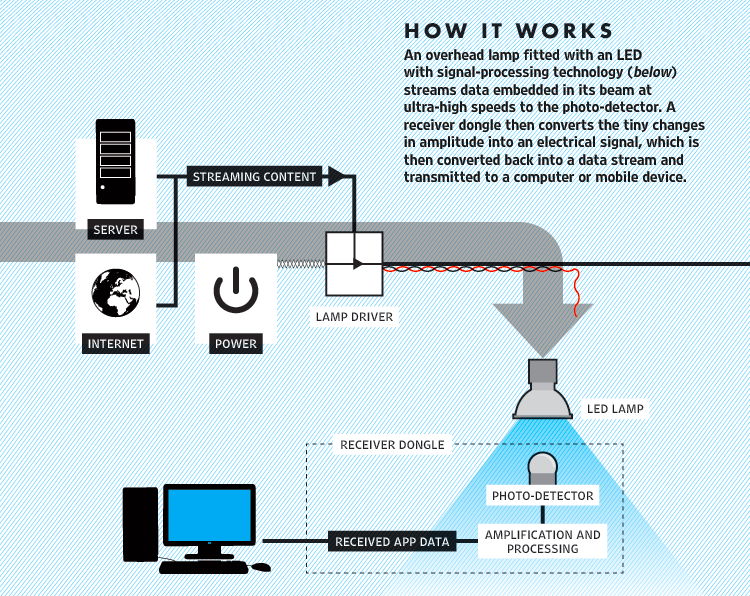
\includegraphics[width=\linewidth]{Kapitel/lifi/Grafiken/How.jpg}
\captionof{figure}{how LiFi works~\cite{lifi.2}}
\label{fig:LiFi_how}
\end{Figure}

\subsubsection*{Eigenschaften}

Li-Fi verfügt über alle Vorteile für die Kapazität, Energieeffizienz und die Sicherheit eines drahtlosen Systems mit einer Reihe von Schlüsselvorteilen die über Wi-Fi hinausgehen (Vgl. \cite{lifi.1}): \\
\begin{itemize}
	\item Bandbreite: \\
		Das sichtbare Lichtspektrum ist groß (10.000x gößer als RF-Spektrum), nicht lizenziert und frei zu verwenden.
	\item Datendichte: \\
		Li-Fi kann ungefähr 1000-fache die Datendichte von Wi-Fi erreichen, weil sichtbares Licht gut in einem engen Beleuchtungsbereich enthalten sein kann, während RF dazu neigt Störungen zu verursachen.
	\item Geschwindigkeit: \\
		In einigen Tests hat LiFi in einer kontrollierten Umgebung Geschwindigkeiten von über 100 Gbps erreicht. Diese 			 	Geschwindigkeiten können durch geringe Störungen erreicht werden (im Vergleich zu Funkfrequenzen ) und eine 				hohe Bandbreite aufgrund des sichtbaren Lichtspektrums , das ist 10.000-mal mehr als das RF-Spektrum, ermöglicht 		eine optimale Benutzerabdeckung, egal wie groß die Anzahl der Benutzer ist.
	\item Planung: \\
		Die Kapazitätsplanung ist einfach, da es häufig dort, wo Menschen kommunizieren wollen, Beleuchtung gibt und 				dann kann eine gute Signalstärke buchstäblich gesehen werden.
	\item Niedrige Kosten:\\
		Erfordert weniger Komponenten als die Funktechnik.
	\item Energie:\\
		LED-Beleuchtung ist bereits sehr Energieeffizient und die Datenübertragung erfordert vernachlässigbar zusätzliche Leistung.
	\item Umwelt:\\
		Der Energieverbrauch  wird durch die Verwendung von LED-Beleuchtung und der erforderten, vernachlässigbaren, zusätzlichen Leistung zur Übertragung von Daten minimiert. Weiterhin ist die RF-Übertragung und Ausbreitung in Wasser extrem schwierig, während Li-Fi auch in dieser Umgebung funktioniert.
	\item Sicherheit:\\
		 Das Leben auf der Erde hat sich durch Belichtung mit sichtbarem Licht entwickelt. Es gibt keine bekannten gesundheitlichen Bedenken für diese Technologie. Die Übertragung von Licht vermeidet die Verwendung von Funkfrequenzen, die elektronische Schaltkreise in bestimmten Umgebungen gefährlich stören könnten. LiFi kommt demnach als Alternative zu den Radiowellen, in sensiblen Umgebungen wie Krankenhäusern, medizinischen Zentren, Schulen, einigen Industrieanlagen in Frage.	
	\item Containment: \\
		Während WiFi-Signale Wände und Decken durchdringen, können LiFi-Signale nur im beleuchteten Bereich empfangen werden, was eine sehr kontrollierbare Umgebung schafft. Die Signale können nicht durch Wände reisen und sind völlig sicher. Es besteht daher keine Gefahr für das LiFi System  durch die Fern-Piraterie. Diese Lösung ist von großem Interesse für sensible Vorgänge wie in der Forschung und Entwicklung, in Verteidigungs- oder Sicherheitssysteme, usw.
		
\item Kontrolle: \\
 Daten können nur von einem Gerät zum anderen geleitet werden, und der Benutzer kann sehen, wo die Daten hingehen. Demnach herrscht keine Notwendigkeit für zusätzliche Sicherheit, wie bspw. Pairing für RF-Verbindungen via Bluetooth.
\end{itemize}
		

\subsection*{Einsatz}
Die Zunahme bei der Verwendung von LEDs für die Beleuchtung bietet die Möglichkeit, Li-Fi -Technologie in einer Vielzahl von LED-Umgebungen zu integrieren.
Li -Fi ist besonders geeignet für Internetanwendungen wie Video- und Audio-Downloads, Live Streaming, o.ä. Diese Anwendungen stellen hohe Anforderungen an die Downlink-Bandbreite, benötigen allerdings nur minimale Uplink-Kapazitäten. Auf diese Weise wird der Großteil des Internetverkehr  von vorhandenen RF -Kanäle abgeladen, was auch die Wi-Fi-Kapazitäten erhöht.
Es gibt viele Anwendungen für Li -Fi. Einige Beispiele sind:
\begin{itemize}
\item RF-Kanal-Entlastung: \\
Kapazitätsanforderungen von Mobilfunknetzen   auf Li-Fi-Netzwerke abgeladen werden. Dies ist besonders dort wirksam, wo Engpässe auf dem Downlink auftreten.
\item Intelligente Beleuchtung: \\ 
Jede private oder  öffentliche LED-Lampe, einschließlich Straßenlampen, kann genutzt kann für Li-Fi-Hotspots genutzt.
\item Mobile Verbindungen: \\
Laptops, Smartphones, Tablets und andere mobile Geräte können mit Li-Fi direkt miteinander verbunden werden. Die kurze Distanz ermöglicht sehr hohe Datenraten und garantiert ebenfalls Sicherheit.
\item Krankenhaus und Gesundheitswesen: \\
Li-Fi emittiert keine elektromagnetischen Störungen und kann so keine medizinischen Instrumente stören.
\item Unterwasserkommunikation: \\ 
Aufgrund starker Signalabsorption im Wasser ist eine RF-Kommunikation impraktikabel und akustische Wellen haben eine extrem geringe Bandweite. Li-Fi bietet auch in dieser Umgebung eine Lösung zur Kurzstreckenkommunikation.
\item Fahrzeuge und Transport: \\ 
LED-Scheinwerfer und Rücklichter von Fahrzeugen können ebenfalls genutzt werden. Auch Straßenlaternen, Schilder und Ampeln können durch LEDs realisiert werden. Dies kann für die Fahrzeug-Fahrzeug- oder Fahrzeug-Straßenrand-Kommunikation genutzt werden, um die Verkehrssicherheit und das Verkehrsmanagement zu verbessern. 
\item Location Based Services: \\
Hochgenaue standortspezifische Informationsdienste wie Werbung und Navigation, ermöglichen den Empfänger  relevante Informationen direkt vor Ort zu erhalten.
\item Spielzeug: \\
Viele Spielzeuge integrieren LED-Leuchten und diese können verwendet werden, um eine äußerst kostengünstige Kommunikation zwischen interaktiven Spielzeug zu ermöglichen.
\end{itemize}

\subsection*{Anbieter und Gremien}


Im Oktober 2011 gründeten Unternehmen und Branchen , das \textit{Li-Fi-Konsortium}, um optische drahtlose High-Speed-Systeme zu fördern und um die begrenzte Menge an funkbasierten Wireless-Spektrum zu überwinden unter der Ausnutzung eines ganz anderen Teils des elektromagnetischen Spektrums.
Das \textit{Li-Fi-Konsortium} hat mehrere Zwecke:
\begin{itemize}
\item Förderung optischer drahtloser Kommunikation bis in Multi- Gigabit-Bereiche in allen Implementierungen
\item Schulung potenzieller Entwickler und Investoren der Unternehmen, um zu helfen deren Produkt- oder Anlageziele zu erreichen
\item Erstellung ganzer Lösungen im Hinblick auf die Kundenbedürfnisse
\item Koordination mit Standardisierungsgruppen und anderen Industrie-Organisationen
\end{itemize}

\end{multicols}
%\newpage
\section*{Historische Entwicklung}
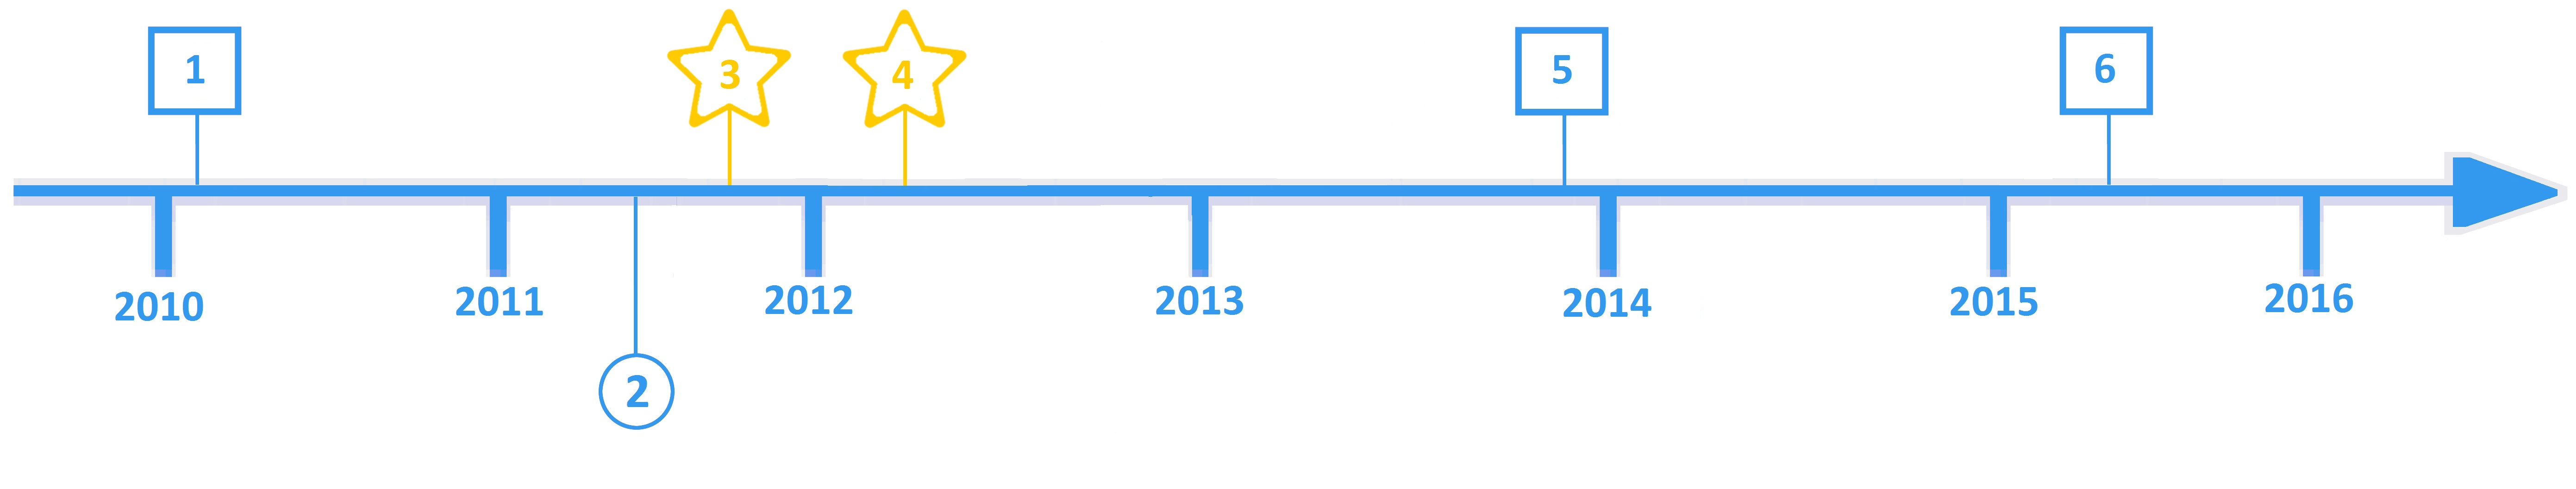
\includegraphics[width=\textwidth]{Kapitel/lifi/Grafiken/Zeitstrahl}
\par
\noindent
\rowcolors{2}{}{\topicolor!20}
\begin{tabular}{p{0.5 cm}p{1.5 cm}p{15.55 cm}}
	Nr. & Datum & Entwicklungsschritte~\cite{lifi.2}\\
	1 & Januar 2010 & Förderung des \textit{D-Light-Project der University of Edinburgh} \\
	2 & Juli 2011 & \textit{TED}- Beitrag "Wireless data from every light"\\
	3 & Oktober 2011 & Gründung des \textit{LiFi-Konsortium}\\
	4 & Januar 2012  & Gründung der \textit{Firma pureLiFi}\\
	5 & August 2013 & Datenrate von 1,6 Gbit/s\\
	6 & 2014 & Datenrate von bis zu 10 Gbit/s \\
\end{tabular}
\par
\begin{multicols}{3}

\textit{Harald Haas}, der an der \textit{University of Edinburgh} in Großbritannien lehrt, prägte den Begriff Li-Fi in seinem Vortrag "Wireless data from every light" während einer \textit{TED}-Diskussion im Juli 2011. Er ist Lehrer für Mobilkommunikation an der \textit{Universität von Edinburgh} und Mitbegründer von \textit{pureLiFi}.

Das \textit{D-Light-Projekt des Edinburgh-Institut für Digitale Kommunikation} wurde von Januar 2010 bis Januar 2012 gefördert. \textit{Haas} förderte diese Technologie in seinem \textit{TED} Beitrag im Jahr 2011 und hat dazu beigetragen, eine Firma zu gründen, die LiFi vermarktet. \textit{PureLiFi} ist ein Unternehmen, das Li-Fi-Produkte in bestehende LED-Beleuchtungssysteme integriert.

Im Oktober 2011, kamen Unternehmen und Industriegruppen zusammen, um ein Li-Fi-Konsortium zu bilden, mit dem Zweck High-Speed-optische drahtlose Systeme zu fördern und die begrenzte Verfügbarkeit an funkbasierten Wireless-Spektrum zu überwinden, unter Ausnutzung eines ganz anderen Teils des elektromagnetischen Spektrums.

Im Jahr 2012 wurde VLC-Technologie ausgestellt, die bereits LiFi nutzte. Im August 2013 wurden Datenraten von bis zu 1,6 Gbit/s mit nur einer einzigen LED-Lampe erzielt. Im Oktober 2013 wurde berichtet, dass bereits chinesische Hersteller an LiFi-Developement-Kits arbeiten.

Im April 2014 kündigte die russische Firma \textit{Stins Coman} die Entwicklung eines Li-Fi, drahtlosen, lokalen Netzwerk namens \textit{BeamCaster} an. Das damals aktuelle Modul übertrugt Daten mit einer Geschwindigkeit von 1,25 Gigabyte pro Sekunde. Im Jahr 2014 wurde ein neuer Rekord von \textit{SiSoft}, einem mexikanischen Unternehmen, eingereicht, das in der Lage war, Daten zu übertragen, bei einer Geschwindigkeiten von bis zu 10 Gbit/s.

\subsection*{Ausblick}
Das Besondere an dieser Technologie ist insbesondere die Einfachheit, mit der die Li-Fi-LED Infrastruktur erstellt und eingesetzt werden kann. Jede Straßenlaterne, jede brennende Autobirne und im Grunde genommen jede Lichtquelle, jede Innen- oder Außenraumbeleuchtung ist damit ein potentieller Träger und ein möglicher Bestandteil der neuen Li-Fi Technologie. All diese Lichtquellen sind potentielle Transportpunkte von Daten und Informationen. Hier ergeben sich gerade für die Autoindustrie wertvolle und außergewöhnliche Einsatzmöglichkeiten. Jede Glühbirne in einem Auto kann Bestandteil eines intelligenten Kommunikationssystems werden. Jede Glühlampe in einem Auto überträgt so die Daten zur nächsten Glühbirne und zum nächsten Auto. Ein unzählbares Netzwerk der Li-Fi Technologie entsteht bei diesen Überlegungen. Daraus ergeben sich unglaublich viele Einsatzmöglichkeiten, welche die Vorstellung derzeit zu sprengen scheinen und alle Gedanken nahezu in Richtung Science Fiction lenken lassen. Li-Fi scheint sich tatsächlich zum neuen Trend der Zukunft zu entwickeln. Hinzu kommt, dass der Sicherheitsaspekt relativ einfach zu berücksichtigen und umzusetzen ist. Schon eine Hauswand kann als ausreichende Abschirmung gelten und dem Datenschutz hinreichende Dienste leisten. Schon stellen Fachleute die ersten Überlegungen an, dass mit der neuen Li-Fi Technologie zukünftig das gesamte Leben und die Kommunikation ohne Kabel möglich werden. Der Entwicklung scheinen keine Grenzen gesetzt

\printbibliography[segment=18,heading=subbibliography]
\end{multicols}
